\section{模型结果}

\subsection{基准特征}

从 eICU 数据库中提取出 $100,308$ 条数据,包含 $17,729$ 名不同的脓毒症患者。%
其中,$3,866\,(3.85\%)$ 条数据为正例,$96,442\,(96.15\%)$ 条数据为反例。

如表 \ref{table:baseline-comparison} 所示,经过比较,%
正例数据拥有更长的 ICU 入住天数、更少的血浆蛋白、更少的淋巴细胞数目、%
更高的心率、更高的呼吸频率、更少的血清总蛋白、更低的红细胞比容、%
更少的肌酸酐、更高的白细胞计数、更多的血小板、更低的平均动脉压。

\begin{table}[htb]
    \centering
    \begin{tabular}{lrrl}
        \toprule
        指标名称    & 正例平均值   & 反例平均值   & 单位                  \\
        \midrule
        ICU入住天数 & 21.067  & 10.852  & 天                   \\
        血浆蛋白    & 2.109   & 2.520   & g/dL                \\
        淋巴细胞数目  & 9.931   & 12.473  & \%                  \\
        心率      & 93.337  & 88.458  & 次/分钟                \\
        呼吸频率    & 21.814  & 21.019  & 次/分钟                \\
        血清总蛋白   & 5.578   & 5.928   & g/dL                \\
        红细胞比容   & 27.808  & 29.888  & $\times 10^3$ K/mcL \\
        肌酸酐     & 1.489   & 1.610   & mg/dL               \\
        白细胞计数   & 13.218  & 12.189  & $\times 10^3$ K/mcL \\
        血小板     & 260.259 & 226.342 & $\times 10^3$ K/mcL \\
        平均动脉压   & 79.727  & 82.055  & mmHg                \\
        \bottomrule
    \end{tabular}
    \caption{正反例基准特征比较($p<0.001$)}
    \label{table:baseline-comparison}
\end{table}

\subsection{模型比较}

\begin{table}[htb]
    \centering
    \footnotesize
    \begin{threeparttable}
        \begin{tabular}{clcc}
            \toprule
            排名 & 模型名称                         & 平均准确率               & 平均AUC\tnote{1}      \\
            \midrule
            1  & CatBoost                     & $0.996 (\pm 0.001)$ & $0.996 (\pm 0.001)$ \\
            2  & Light Gradient Boosting      & $0.995 (\pm 0.001)$ & $0.996 (\pm 0.001)$ \\
            3  & Extreme Gradient Boosting    & $0.995 (\pm 0.001)$ & $0.994 (\pm 0.002)$ \\
            4  & Hist Gradient Boosting       & $0.994 (\pm 0.002)$ & $0.996 (\pm 0.002)$ \\
            5  & Ada Boost                    & $0.993 (\pm 0.002)$ & $0.995 (\pm 0.002)$ \\
            6  & Decision Tree                & $0.989 (\pm 0.002)$ & $0.949 (\pm 0.013)$ \\
            7  & Multi-Layer Perceptron       & $0.982 (\pm 0.004)$ & $0.975 (\pm 0.008)$ \\
            8  & SVM (RBF Kernel)             & $0.973 (\pm 0.003)$ & $0.957 (\pm 0.011)$ \\
            9  & Logistic                     & $0.966 (\pm 0.007)$ & $0.956 (\pm 0.012)$ \\
            10 & Extra Trees                  & $0.961 (\pm 0.006)$ & $0.977 (\pm 0.006)$ \\
            11 & Naive Bayes                  & $0.961 (\pm 0.006)$ & $0.689 (\pm 0.034)$ \\
            12 & Ridge                        & $0.961 (\pm 0.007)$ & $0.952 (\pm 0.013)$ \\
            13 & Linear Discriminant Analysis & $0.961 (\pm 0.010)$ & $0.952 (\pm 0.013)$ \\
            14 & K-Nearest Neighbours         & $0.951 (\pm 0.006)$ & $0.544 (\pm 0.025)$ \\
            \bottomrule
        \end{tabular}
        \begin{tablenotes}
            \tiny
            \item[1] AUC:Area Under Curve,接受者操作特性曲线下与坐标轴围成的面积。
        \end{tablenotes}
    \end{threeparttable}
    \caption{$14$种模型的交叉验证结果比较(按平均准确率排序)}
    \label{table:model-comparison}
\end{table}

用提取出的数据训练预测模型,各种模型的交叉验证结果如表 \ref{table:model-comparison} 所示。%
Logistic 回归表现良好(平均准确率:$0.966$ ,平均 AUC :$0.956$),%
而集成学习方法拥有更高的平均准确率和平均 AUC 。%
其中,CatBoost 的预测结果最好(平均准确率:$0.996$ ,平均 AUC:$0.996$),%
故选择 CatBoost 进入下一步。

\subsection{完整模型与紧凑模型}

\begin{figure}[htb]
    \centering
    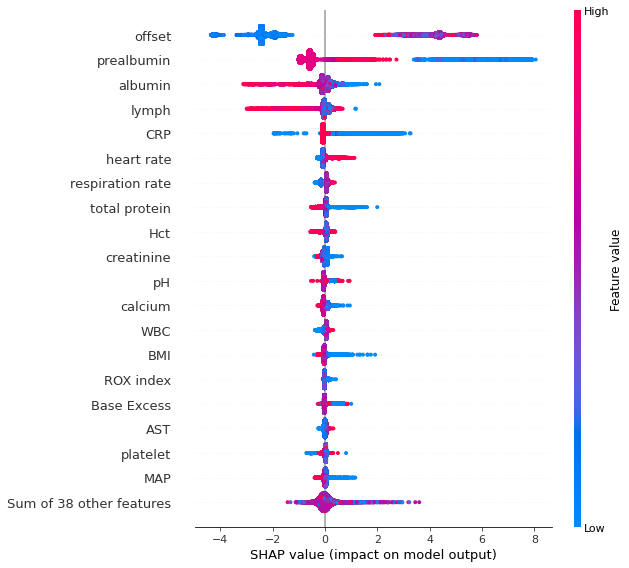
\includegraphics[width=0.9\linewidth]{../img/eicu_full_shap_beeswarm_20.png}
    \caption{完整模型中各变量的平均 SHAP 值比较}
    \label{figure:full-shap}
\end{figure}

根据预测结果比较,选择含 $57$ 个输入变量的 CatBoost 模型为完整模型。%
计算完整模型中各变量的平均 SHAP 值,结果如图 \ref{figure:full-shap} 所示。%
此摘要图展示了各个变量对预测结果的影响情况分布。%
例如,ICU 入住天数(offset)对结果影响明显,且 ICU 入住天数越长,发生ICU综合症的概率越大。

根据变量的平均 SHAP 值大小和数据获取的难易程度,选择了 $15$ 个变量作为输入,%
建立更加易于使用的紧凑模型。使用默认超参数的紧凑模型平均AUC为 $90.219\%$ 。%
用贝叶斯优化调整超参数后,紧凑模型平均 AUC 达到了 $90.682\%$ ,同时平均准确率为 $96.120\%$ 。%
虽然预测结果的得分略低于完整模型,但是紧凑模型明显在临床上更加可行、更加易用。

\subsection{性能分析}

\begin{figure}[htb]
    \centering
    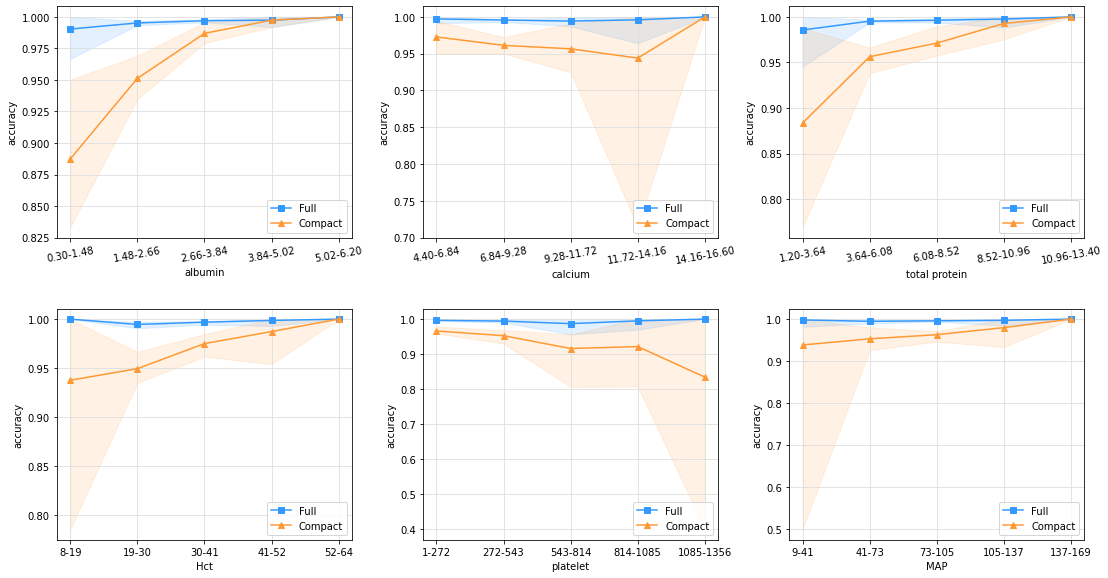
\includegraphics[width=\linewidth]{../img/eicu_performance.png}
    \caption{模型性能分析}
    \label{figure:model-performance}
\end{figure}

如图 \ref{figure:model-performance} 所示,完整模型和紧凑模型在各种指标的不同范围下都表现良好。%
当某个指标出现明显的异常值时,模型可以非常敏锐地察觉到并给出十分准确的预测结果。

\subsection{模型解释}

\begin{figure}[htb]
    \centering
    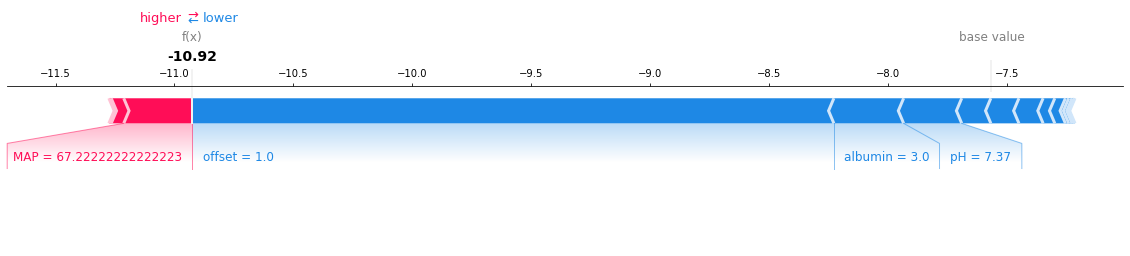
\includegraphics[width=\linewidth]{../img/eicu_compact_shap_force_neg.png}
    \vspace{-4em}
    \caption{个例(A)中主要变量的 SHAP 值}
    \label{figure:shap-neg}
\end{figure}

\begin{figure}[htb]
    \centering
    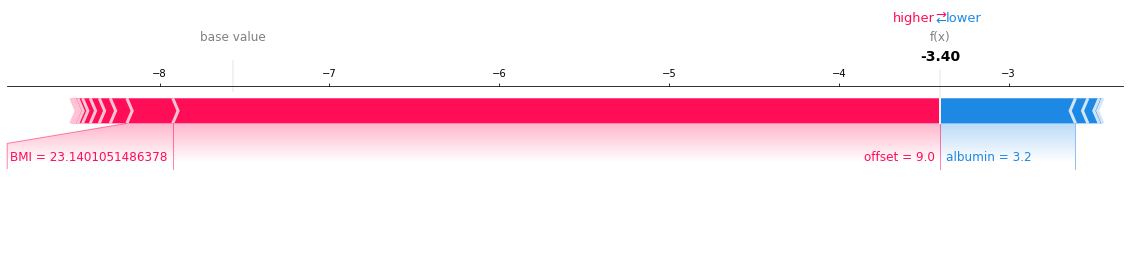
\includegraphics[width=\linewidth]{../img/eicu_compact_shap_force_pos.png}
    \vspace{-4em}
    \caption{个例(B)中主要变量的 SHAP 值}
    \label{figure:shap-pos}
\end{figure}

图 \ref{figure:full-shap} 从整体上展示了各个变量对于预测结果的影响情况,%
同时也展现了模型对输入变量变化的灵敏性。%
而图 \ref{figure:shap-neg} 和图 \ref{figure:shap-pos} 展示了两个个例(主)变量的 SHAP 值。%
图中红色条和蓝色条分别表示危险因素和安全因素,它们共同作用决定了最终的结果。%
如图 \ref{figure:shap-neg} ,在个例(A)中,虽然患者的平均动脉压偏低,但是其 ICU 入住天数很短、%
血浆蛋白较多、pH 值也良好,所以模型准确预测了患者次日无 ICU 综合症风险。%
又如图 \ref{figure:shap-pos} ,在个例(B)中,虽然患者的血浆蛋白较多,%
但是其 ICU 入住天数较长、身体质量指数(BMI)偏低,所以模型准确预测了患者次日的 ICU 综合症。

\subsection{H5预测工具}

\newcommand\PredictionToolURL{http://1.15.185.22/sepsis-pics-tool/}

为了方便临床上对上述紧凑模型的测试,开发了一款预测脓毒症患者诱发 ICU 综合症的 H5 应用。%
只需在表单中输入指标数值,然后点击“提交”,就可以获得紧凑模型对患者次日发生 ICU 综合症概率的预测。%
目前应用已部署在此网址上:\url{\PredictionToolURL} 。
